\documentclass[11pt]{article}

\title{Dimensionality reduction \\ - \\ Concepts, and applications in scRNA-seq and DNA microscopy}
\author{Gergo Bohner}

\usepackage{graphicx}
\graphicspath{{fig/}}

\usepackage{hyperref}

\usepackage{amssymb}

\begin{document}

\maketitle


\section{The goals of dimensionality reduction}

Dimensionality reduction is a widely applied set of methods in various data analysis pipelines. It has three main aims:

\begin{itemize}
	\item \emph{Describe the data manifold} \\ Parametrise a space that we believe the observed data lives in. This space also serves as generalisation of where we expect future data to show up. Furthermore certain parameterisations  may facilitate interpretation of features.
	\item \emph{Reduce the observation noise} \\ We may separate the data variance into "within-manifold" (signal) and "out-of-manifold" (noise), this is called variance partitioning. Often only the within-manifold signal is used for further processing.
	\item \emph{Visualise the concepts discovered in the data} \\ Most collected data nowadays is very high (100+) dimensional, whereas most humans can only conceptualise a few dimensions at once. We have the responsibility to choose the most effective, yet accurate visualisations of the data to communicate features of the data - which may be even more informative together with information derived otherwise (such as derived clusters or external information).
\end{itemize} 



\subsection{Examples of specific goals}

Finding pure examples of specific dimensionality reduction applications is difficult, as dimensionality reduction methods are often used in conjunction with other techniques to communicate ideas. In the next few pages I show examples of well-defined, distinct applications of various dimensionality reduction methods, to help clarify the breadth of goals we may think of.
 
 \clearpage
 
\subsubsection{Manifold learning} 
(e.g. Isomap, LLE) \\ Estimate within-manifold distances, predict what data is likely in the future, learn about structure embedded within the data
 

\begin{figure}[h!]
\centering
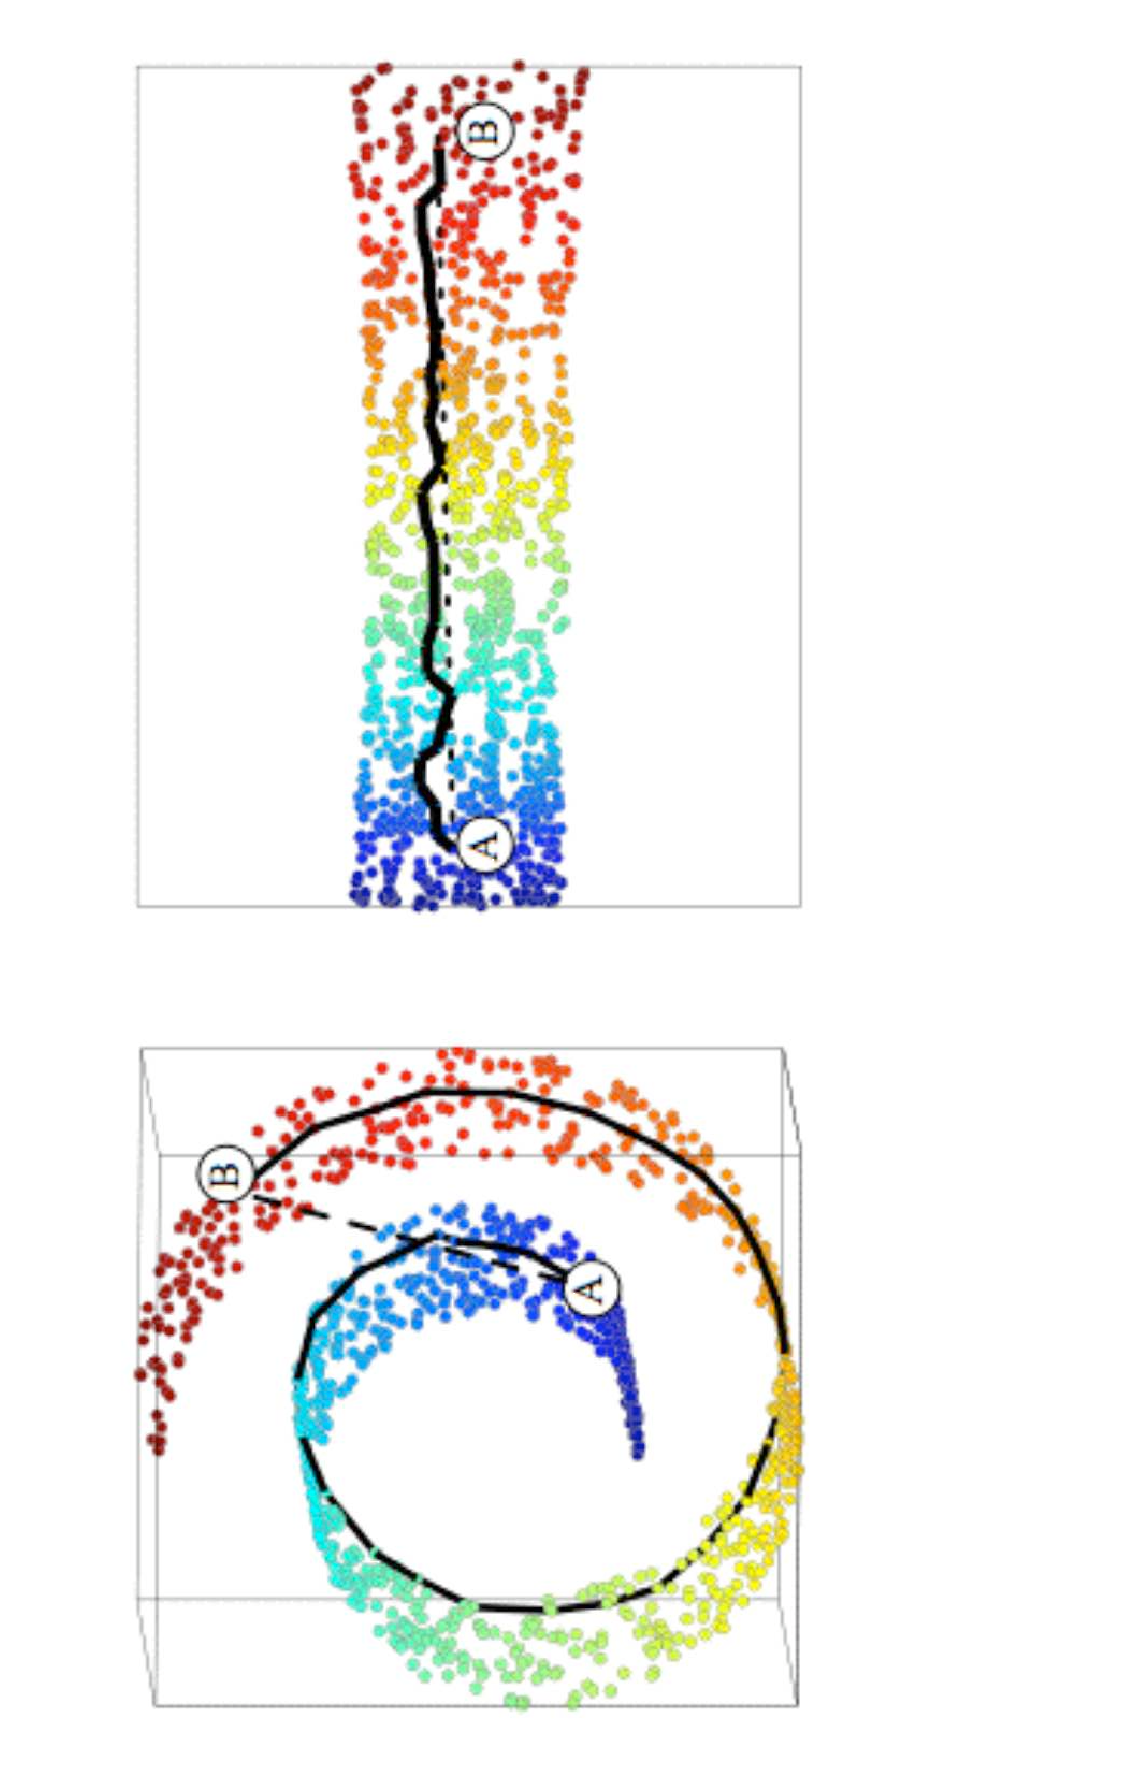
\includegraphics[angle=-90,origin=c, height=0.7\linewidth, width=0.73\textwidth]{swiss-unroll-distance}
\\ \vspace{-3cm}
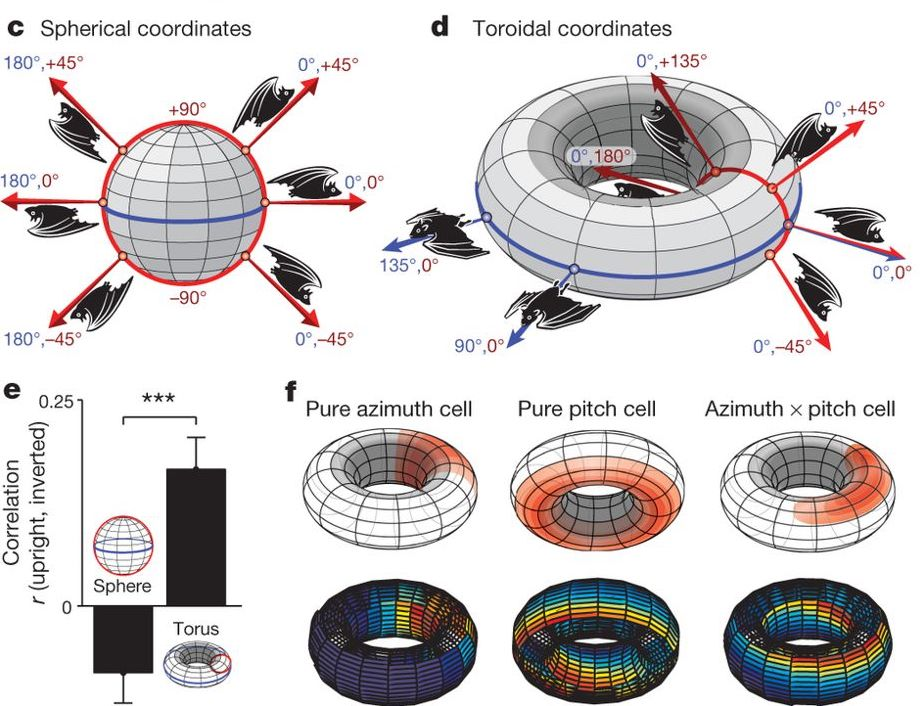
\includegraphics[width=0.5\linewidth]{bat_neurons_nature14031-f3} 
\caption{Examples for manifold estimation. (top) Swiss roll artificial dataset shows the concepts of a 2D manifold embedded in 3D (color purely serves as visual aid). (bottom) Comparing different manifold hypotheses (spherical vs toroidal) in behaving bats to explain neural variability \emph{(Finkelstein et al, Nature 2015)}}
\end{figure} 

\clearpage

 
\subsubsection{Feature discovery} 
(e.g. PCA, ICA, NMF) \\ Find a meaningful "basis" for the manifold - a set of features whose combination explains the data well, and leads to investigable hypotheses about the building blocks of the phenomenon that resulted in the collected data. 
 

\begin{figure}[h!]
\centering
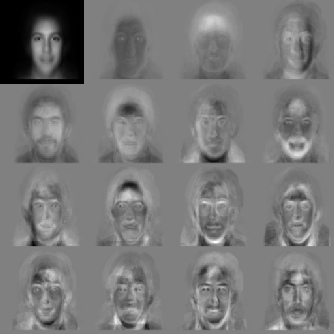
\includegraphics[width=0.5\linewidth]{eigfacessmall}
\caption{Example feature discovery - Given a corpus of grayscale face portraits, find the "average" face, and the main directions of variation (in pixel space). Note that even though the principal components are shown as 2D images, in reality the spatial structure is purely due to actual structure in the data, the algorithm was not looking for it (like convolutional neural nets explicitly do). }
\end{figure} 

\clearpage

 
\subsubsection{Reduce observation noise} (e.g. PCA, pPCA, FA, projection on manifold) \\ Experimenters can assume various sources of noise that is corrupting their input data, and select the appropriate method that is capable of separating signal from noise.
 

\begin{figure}[h!]
\centering
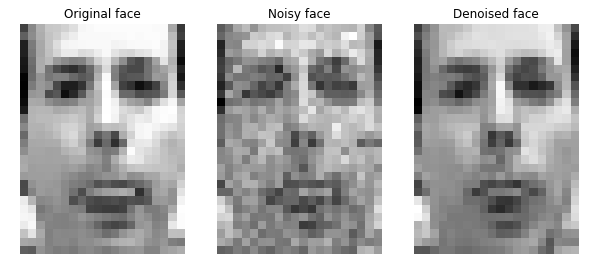
\includegraphics[width=0.75\linewidth]{pca_denoising_frey}
\\
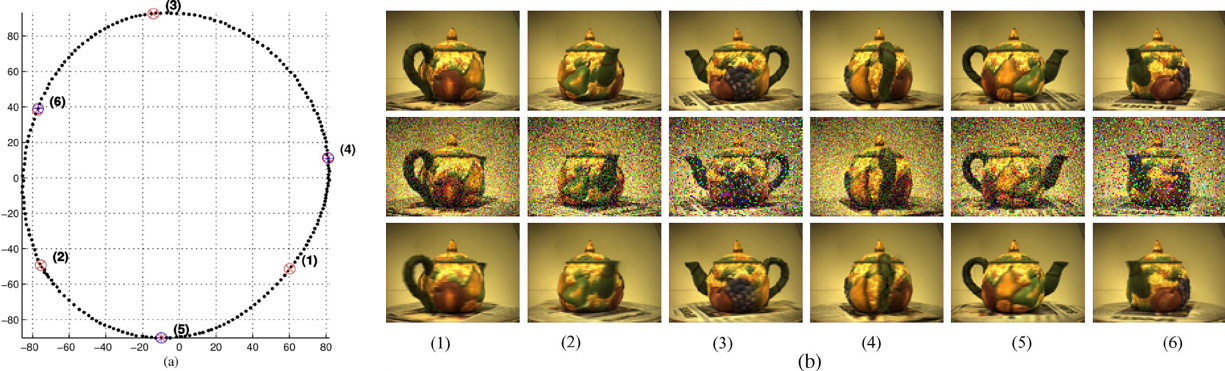
\includegraphics[width=1.0\linewidth]{nonlinear_denoising_teapot_cropped}
\caption{Denoising examples - (top) Using PCA to reduce the effects of additive, uniform and identically distributed Gaussian noise (PCA is optimal for this kind of noise). (bottom) Nonlinear manifold-based associative image denoising. Rotating teapot images embedded in low-D space (a), projection on learned manifold results in noise free images (b). \emph{Huang et al. Manifold-Based Learning and Synthesis} \url{doi 10.1109/TSMCB.2008.2007499}}
\end{figure} 

\clearpage

 
\subsubsection{Visualise high-D data via non-linear embedding} 
(e.g. LLE, Isomap, t-SNE) \\ Many dimensionality reduction methods have no easy-to-understand concepts in either a) what features of the high dimensional data they wish to keep unchanged in the low dimensional embedding or b) how they map from the high dimensional space to the low dimensional. \\ \\ Yet many of them become popular due to their ability to create embeddings in which humans may discover structure in, despite the lack of mathematical guarantees. These methods should be exclusively used for data visualisation, and to only communicate features or concepts of the data that have already been confirmed by other means (such as external information or clustering).
 

\begin{figure}[h!]
\hspace{-2cm}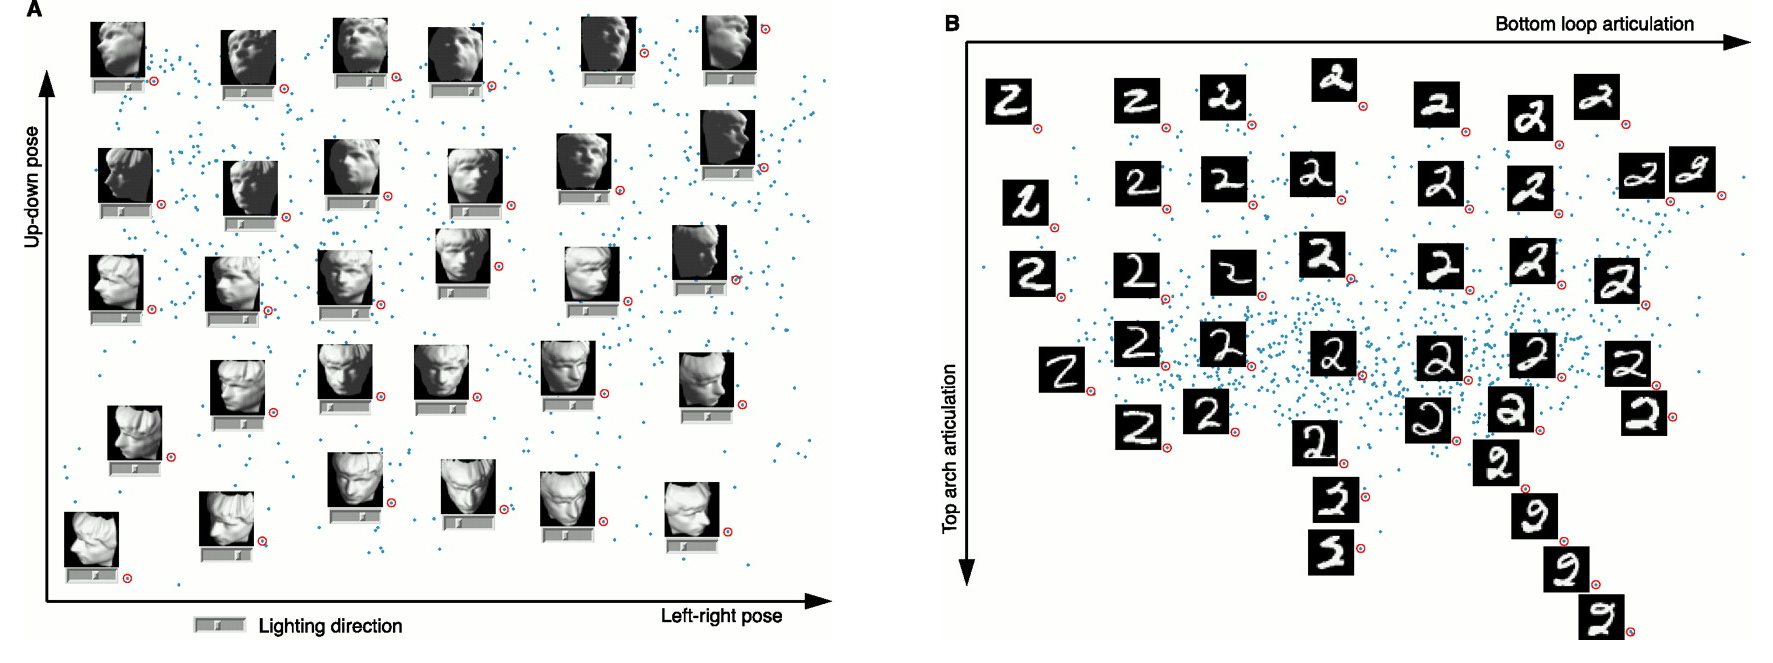
\includegraphics[width=1.3\linewidth]{isomap-head-digit-embeddings-2}

\caption{Visualising high-D data via isomap - Datasets can easily be projected into 3D (left) or 2D (right) spaces. Humans can then look at how samples change in the embedding space, and come up with interpretations for the axes. However, these interpretations then need to be treated as hypothesis, translated back into provable mathematical definitions, and shown to be supported by the data. \emph{J. B. Tenenbaum et al. ISOMAP - A Global Geometric Framework for Nonlinear Dimensionality Reduction} \url{http://web.mit.edu/cocosci/isomap/isomap.html}}
\end{figure} 

\clearpage

\subsection{Example of interspersed goals}

Most often dimensionality reduction methods will serve multiple of the above goals at once, usually combining visualisation of high-D data, feature discovery and communicating of additional meta-data or concepts discovered via other methods (such as coloring by cluster identity).

\begin{figure}[h!]
\begin{center}
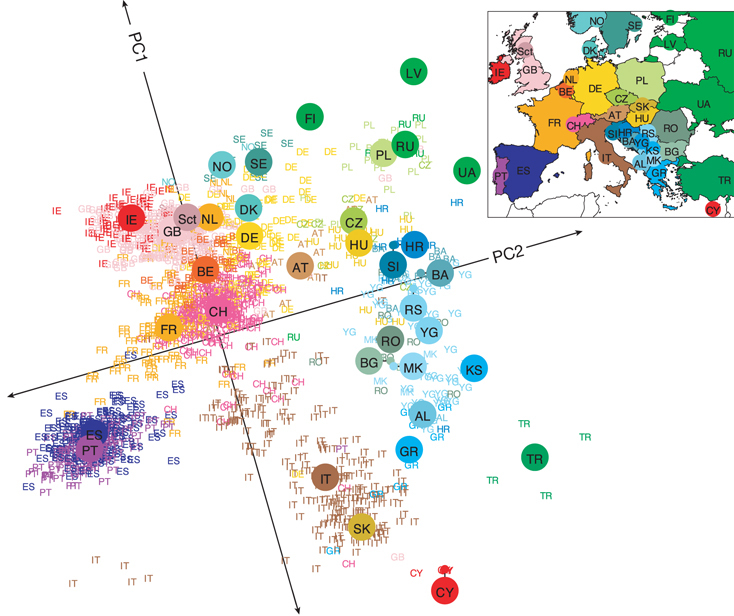
\includegraphics[width=0.62\linewidth]{genetics-pca-europe-map}\hspace{-1cm}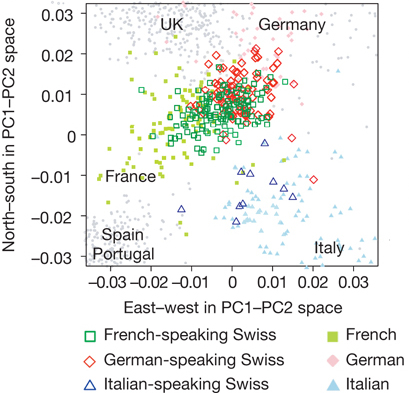
\includegraphics[width=0.32\linewidth]{genetics-pca-europe-swiss}

\vspace{0.5cm}
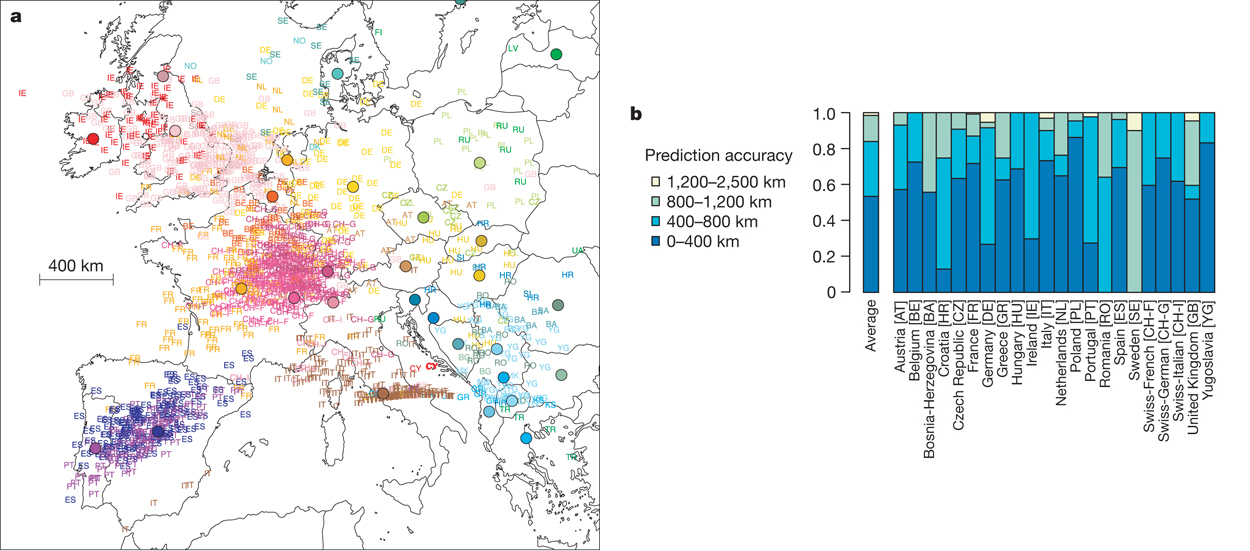
\includegraphics[width=0.75\linewidth]{genetics-pca-europe-cvpred}
\caption{Interspersed goal - Communicating PCA embedding to 2D, cluster identity (from metadata) and geographical matching in the same figure. (top) PCA embedding of genetic sequencing data, in 2D, colored by nationality, cluster center of masses indicated. (top, inset) zoom in on Swiss population, colored by mother-tongue. (bottom) geographical prediction accuracy of sample location, split by country.  }
\end{center}
\end{figure} 

\clearpage

\section{Mathematical concepts}

\subsection{Linear methods}
(PCA, MDS)

The primary linear methods for dimensionality reduction are PCA (Principal component analysis) and MDS (Multi-dimensional scaling). They are both matrix factorisation methods, but may be applied to different statistics of the input dataset (PCA acts on the scatter matrix [scaled covariance matrix], whereas MDS acts on the Gram matrix [a set of similarity measures]). 

Data points should be thought of as $D_x$ x $1$ column vectors (even images, if my image dimensions are $w$ x $h$, for these methods I just think of them as a single vector with $D_x = w*h$).

A collection of data points can thus be represented as a matrix, where each column is a data point

$$ X \in \mathbb{R}^{D_x\times N} $$

$$ x_i = X[:,i] $$





\end{document}
